\documentclass{beamer}

\usepackage[utf8]{inputenc}
\usepackage{czech}
\usepackage{graphicx}
\usepackage{amsmath}
\usepackage{amsfonts}
\usepackage{amssymb}
\usepackage{hyperref}
\usepackage{tikz}

\usetheme{Frankfurt}

\newtheorem*{question}{Otázka}
\newtheorem*{response}{Odpověď}
\newtheorem*{motivation}{Motivace}
\newtheorem*{taskspec}{Zadání}
\newtheorem*{rulespec}{Pravidlo}
\newtheorem*{rulemathspec}{Specifikace pravidla}
\newtheorem*{graphmodel}{Grafový model}

\title{Validace principů objektového návrhu v~kódu}
\author{Martin Vejmelka}

\linespread{1.3}

\begin{document}

\begin{frame}
  \titlepage
\end{frame}

\begin{frame}
  \tableofcontents
\end{frame}

\section{Motivace a zadání práce}
\begin{frame}
  \frametitle{Motivace projektu}
  \begin{figure}[h!]
    \centering
    \scriptsize
    \begin{tikzpicture}[scale=0.7]
      \shadedraw  (0,0) rectangle (4,4);
      \shadedraw  (4.2,0) rectangle (8.2,4);
      \draw  (0,4.2) rectangle (4.0,8.2);
      \draw  (4.2,4.2) rectangle (8.2,8.2);

      \draw  (2,2) node[text width=2.5cm, text centered] {množina pravidel};
      \draw  (6.2,2) node[text width=2.5cm, text centered] {instance splňující pravidla};
      \draw  (2,6.2) node[text width=2.5cm, text centered] {gramatika a standardní knihovny};
      \draw  (6.2,6.2) node[text width=2.5cm, text centered] {instance jazyka generovaného gramatikou};

      \draw (-2,2) node[text width=2.5cm, text centered] {kódové konvence (těžko vynutitelné)};
      \draw (-2,6.2) node[text width=2.5cm, text centered] {definice programovacího jazyka};

      \draw (2,8.6) node[text width=2.5cm, text centered] {meta-model};
      \draw (6.2,8.6) node[text width=2.5cm, text centered] {model};
    \end{tikzpicture}
  \end{figure}


\end{frame}

\begin{frame}
  \frametitle{Zadání práce}
  \textit{Seznamte se se základními principy používanými při objektově orientovaném návrhu a implementaci, konkrétně s low coupling, high cohesion a Law of Demeter. Popište pravidla, která umožní ověřování těchto principů. Vytvořte nástroj, který umožní analyzovat kód v jazyce Java a vyhodnocovat vámi definovaná pravidla. Činnost nástroje ověřte na vzorových příkladech kódu. Při návrhu nástroje se zaměřte na jeho budoucí rozšiřitelnost.}
\end{frame}

\begin{frame}
  \frametitle{Zadání práce - dekompozice}
  Zadání práce bylo dekomponováno na následující části:
  \begin{itemize}
  \item rešerše souvisejících prací, seznámení se s principy objektově orientovaného návrhu, analýza problémové domény
  \item návrh formalizace popisu pravidel objektově orientovaného návrhu
  \item realizace nástroje pro vyhodnocování pravidel popsaných v navrženém formalismu
  \item testování výsledného řešení na vzorových příkladech kódu
  \end{itemize}
\end{frame}

\section{Analýza}
\begin{frame}
  \frametitle{Analýza}
  \begin{itemize}
  \item průzkum existujících řešení
  \item analýza návrhových konceptů a principů
  \item analýza problémové domény
    \begin{itemize}
    \item analýza vstupů -- projekty v jazyce Java
    \item rešerše nástrojů pro předzpracování kódů do vhodné podoby
    \end{itemize}
  \end{itemize}
\end{frame}

\section{Návrh formalizace pravidel}
\begin{frame}
  \frametitle{Návrh formalizace pravidel}
  \only<1> {
    \begin{graphmodel}
      \begin{displaymath}
        G = \langle V, E, \rho, K, C, N, \mathit{Kind}, \mathit{Classifier}, \mathit{Name}\rangle
      \end{displaymath}
      \tiny
      \begin{itemize}
      \item $V$ je množina elementů (v~našem případě části kódu),
      \item $E$ je množina hran (v~našem případě vztahy mezi částmi kódu -- např. volání funkce, dědičnost),
      \item $V \cap E = \emptyset$,
      \item $\rho: E \mapsto V \times V$ je zobrazení množiny hran do množiny uspořádaných dvojic vrcholů (incidence),
      \item $K$ je libovolná množina označení typů vrcholů,
      \item $C$ je množina klasifikátorů hran,
      \item $N$ je množina jmen (řetězců),
      \item $\mathit{Kind}: V \mapsto K$ je zobrazení, které přiřadí každému vrcholu jeho typ,
      \item $\mathit{Classifier}: E \mapsto C$ je zobrazení, které přiřadí každé hraně její klasifikátor (zda se jedná o~vyvolání metody, dědičnost, apod.),
      \item $\mathit{Name}: V \mapsto N$ je zobrazení, které přiřadí vrcholu jeho jméno (např. jméno třídy, jméno metody).
      \end{itemize}
    \end{graphmodel}
  }
  \only<2> {
    \begin{rulespec}
      Pro počet parametrů $n$ každé metody platí $n \leq 2$.
    \end{rulespec}
    \begin{rulemathspec}
      \begin{align*}
        \forall v \in V &: HasKind(v, ``method") \\
        \\
        CountLessThan&(OutgoingEdges(v, ``param"), 2)
      \end{align*}
    \end{rulemathspec}
  }
  \only<3> {
    \begin{figure}[h!]
      \centering
      \includegraphics[width=1.0\textwidth]{./graphs/graph_example1.png}
      \caption{Příklad grafového modelu.}
    \end{figure}
  }
  \only<4> {
    \begin{figure}[h!]
      \centering
      \includegraphics[width=1.0\textwidth]{./graphs/graph_example2.png}
      \caption{Výběr vrcholů: $\forall v \in V : HasKind(v, ``method")$.}
    \end{figure}
  }
  \only<5> {
    \begin{figure}[h!]
      \centering
      \includegraphics[width=1.0\textwidth]{./graphs/graph_example3.png}
      \caption{Výběr množiny hran: $OutgoingEdges(v, ``has\_param")$.}
    \end{figure}
  }
  \only<6> {
    \begin{figure}[h!]
      \centering
      \includegraphics[width=1.0\textwidth]{./graphs/graph_example4.png}
      \caption{Chyba: $CountLessThan(OutgoingEdges(v, ``has\_param"), 2)$.}
    \end{figure}
  }
\end{frame}

\section{Realizace vyhodnocovacího nástroje}
\begin{frame}
  \frametitle{Realizace vyhodnocovacího nástroje - architektura}
  \begin{itemize}
    \item \emph{GraphModel} -- množina grafů různých typů pro analyzovaný projekt
    \item \emph{ValidationModel} -- stromová struktura pravidel (operátorů) vygenerovaná z AVD souborů
    \item \emph{AVD} -- ArchVal Definitions -- DSL pro serializaci matematických pravidel
    \item \emph{body rozšíření systému}
    \begin{itemize}
      \item operátory (predikáty, selektory)
      \item analýzy
      \item generátory grafů
    \end{itemize}
  \end{itemize}
\end{frame}

\begin{frame}
  \frametitle{Realizace vyhodnocovacího nástroje - editor AVD}
    \begin{figure}[h!]
      \centering
      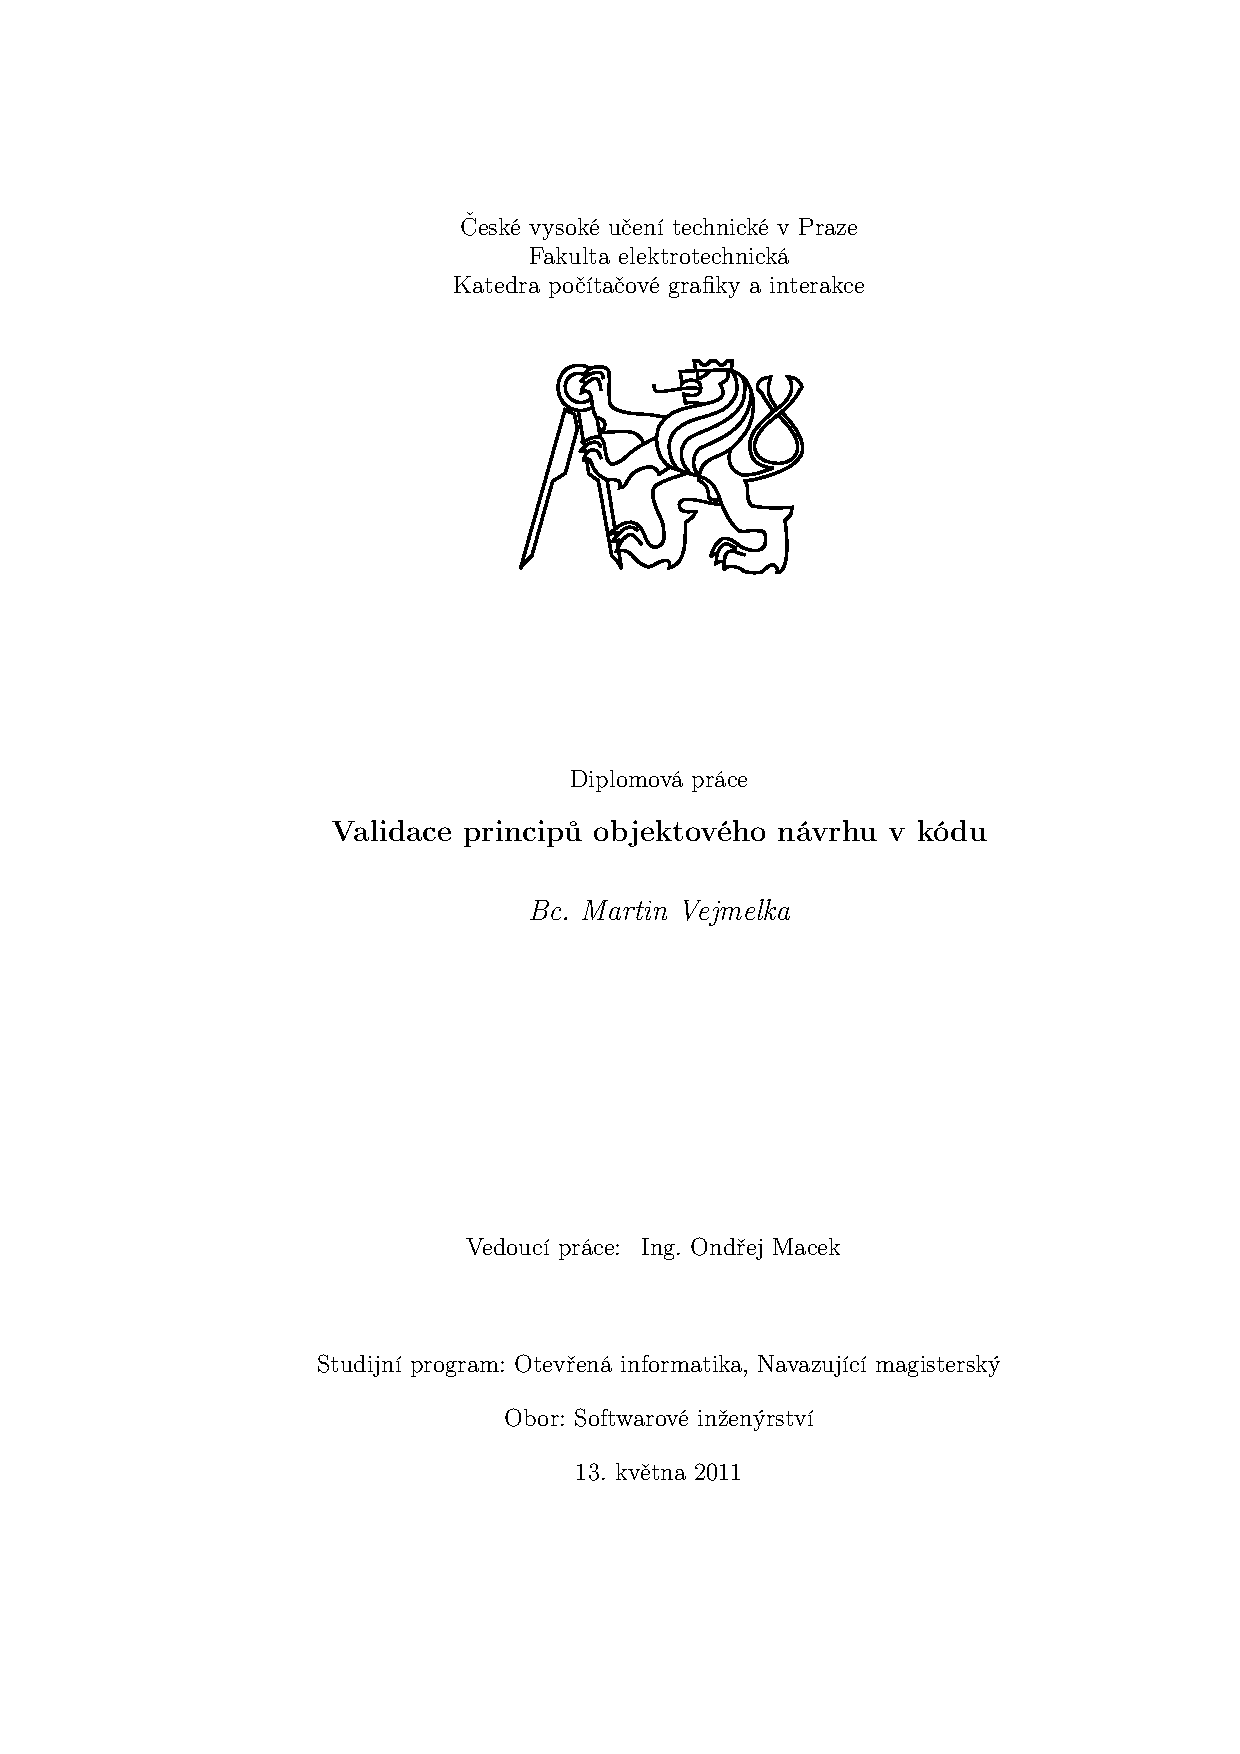
\includegraphics[width=1.0\textwidth]{./figures/archval.png}
    \end{figure}
\end{frame}

\section{Závěr}
\begin{frame}
  \frametitle{Závěr}
  \begin{itemize}
  \item použití běžného matematického zápisu pro formalizaci pravidel
  \item rozšiřitelný nástroj pro vyhodnocování pravidel v zavedeném formalismu
  \item proof of concept - realizace pravidla Law of Demeter
  \item otestování práce na vzorových příkladech
  \end{itemize}
\end{frame}

\section{Otázky}
\begin{frame}
  \frametitle{Otázky}
  \begin{question}
    Jak hodnotíte váš nástroj v porovnání s obdobnými nástroji uvedenými v analytické části práce?
  \end{question}
  \begin{response}
    \begin{itemize}
    \item zmíněné nástroje jsou vyspělejší a dobře integrované do vývojových IDE,
    \item existující nástroje nezavádí matematický přístup k formalizaci pravidel (poskytují předdefinované množiny pravidel),
    \item práce neměla (alespoň prozatím) za cíl konkurovat existujícím nástrojům, ale vyzkoušet nový/jiný přístup.
    \end{itemize}
  \end{response}
\end{frame}

\begin{frame}
  \frametitle{Otázky}
  \begin{question}
    Je možné některý z nástrojů upravit tak, aby byl schopný pracovat s navrženým způsobem ověřování?
  \end{question}
  \begin{response}
    \begin{itemize}
    \item jádro vyvinutého nástroje nemá přímé závislosti na konkrétní platformě,
    \item nutnost poskytnout kompletní grafový model, případně i přídatné operátory,
    \item možnost využít platformu poskytovanou touto prací.
\end{itemize}
  \end{response}
\end{frame}

\begin{frame}
  \frametitle{Otázky}
  \begin{question}
    Nebylo možné použít některý ze stávajících formalismů (např. Featherweight Java) pro popis pravidel?
  \end{question}
  \begin{response}
    \begin{itemize}
    \item nástroj je realizován na vyšší úrovni abstrakce,
    \item pravidla jsou definována nad obecným grafovým modelem,
    \item FJ by určitě bylo možné využít -- jako elementy v pravidlech by vystupovaly elementy jazyka FJ (příp. FGJ),
    \item pro exaktní formalizaci bychom zvolili vhodné zobrazení programu ve FJ do grafu,
    \item nástroj pracuje nad programy v jazyce Java ($FJ \subset Java$).
    \end{itemize}
  \end{response}
\end{frame}

\begin{frame}
  \frametitle{Otázky}
  \begin{question}
    Chybějící formální sémantika formátu AVD.
  \end{question}
  \begin{response}
    \begin{itemize}
    \item AVD je pouze serializací zápisu pravidel popsaných v práci,
    \item jednalo se o nástroj jak vložit pravidla pro testování ve vhodné podobě do počítače (proof of concept),
    \item v případě budoucího rozvoje práce je určitě vhodné rozšířit existující ANTLR gramatiku o popis významu jednotlivých konstruktů.
    \end{itemize}
  \end{response}
\end{frame}

\begin{frame}
  \begin{center}
    {\huge Děkuji za pozornost\ldots}
  \end{center}
\end{frame}

\end{document}
